\section{Connection}
I dette afsnit beskrives designet af systemets klient og server, der sammen udgør den del af systemet som kaldes connection. Forbindelsen mellem de 2 dele, bygger på TCP/IP sockets. Der er valgt ikke selv at designe forbindelsen fra bunden, da der findes eksempler på https://msdn.microsoft.com/en-us/library/w89fhyex(v=vs.110).aspx ??. Af disse er udvalgt et eksempel på en Synchronous Socket Client og en Asynchronous Socket Server. Forskellen i disse er hvor vidt de blokkerer udførslen af programmet når der oprettes en socket. På server siden ønskes at der kan oprettes flere forbindelser på samme tid, hvorimod der på klienten kun oprettes en enkelt forbindelse. Derfor er klienten synchronous, mens serveren er asynchronous.

Klient struktur ses i UML diagram på figur~\ref{fig:ConnectionClient}
\begin{figure}
	\centering
	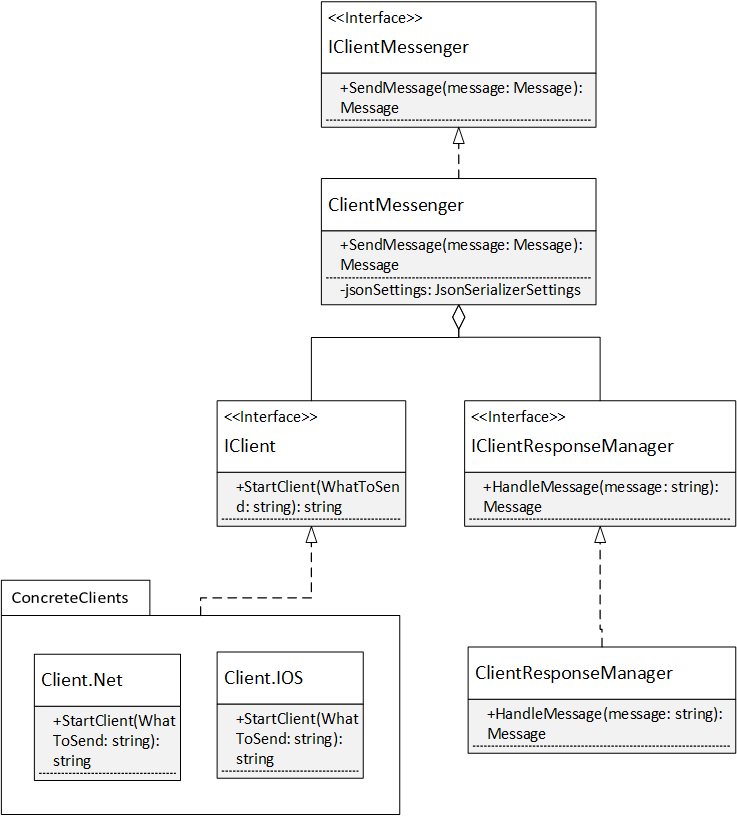
\includegraphics[width=0.9\linewidth]{figs/connection/ConnectionClient.png}
	\caption{Klient diagram}
	\label{fig:ConnectionClient}
\end{figure}

Et typisk forløb i klienten er vist på figur~\ref{fig:ClientSequence}
\begin{figure}
	\centering
	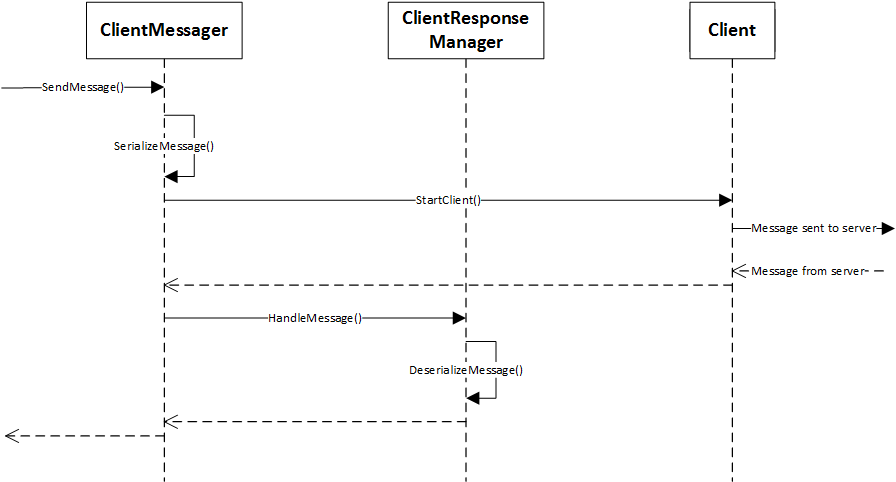
\includegraphics[width=0.9\linewidth]{figs/connection/ClientSequence.png}
	\caption{Client Sequence Diagram}
	\label{fig:ClientSequence}
\end{figure}

Server struktur ses i UML diagram på figur~\ref{fig:ConnectionServer}
\begin{figure}
	\centering
	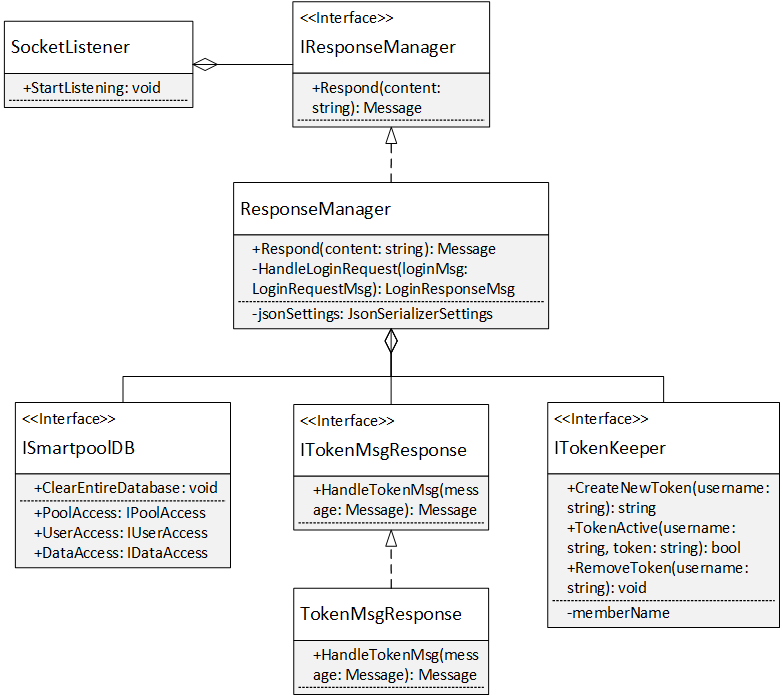
\includegraphics[width=0.9\linewidth]{figs/connection/ConnectionServer.png}
	\caption{Server diagram}
	\label{fig:ConnectionServer}
\end{figure}

Et typisk forløb i serveren er vist på figur~\ref{fig:ServerSequenceResponse}
\begin{figure}
	\centering
	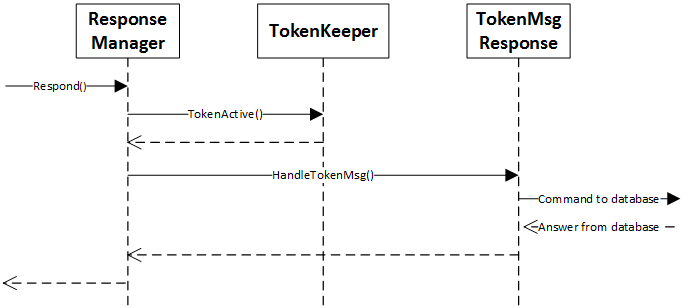
\includegraphics[width=0.9\linewidth]{figs/connection/ServerSequenceResponse.png}
	\caption{Server Sequence Diagram}
	\label{fig:ServerSequenceResponse}
\end{figure}

For at lave et user session koncept, er der implementeret et token system, som består af en TokenKeeper, Token og TokenStringGenerator klasse. UML diagram over disse ses på figur~\ref{fig:ConnectionServerToken}
\begin{figure}
	\centering
	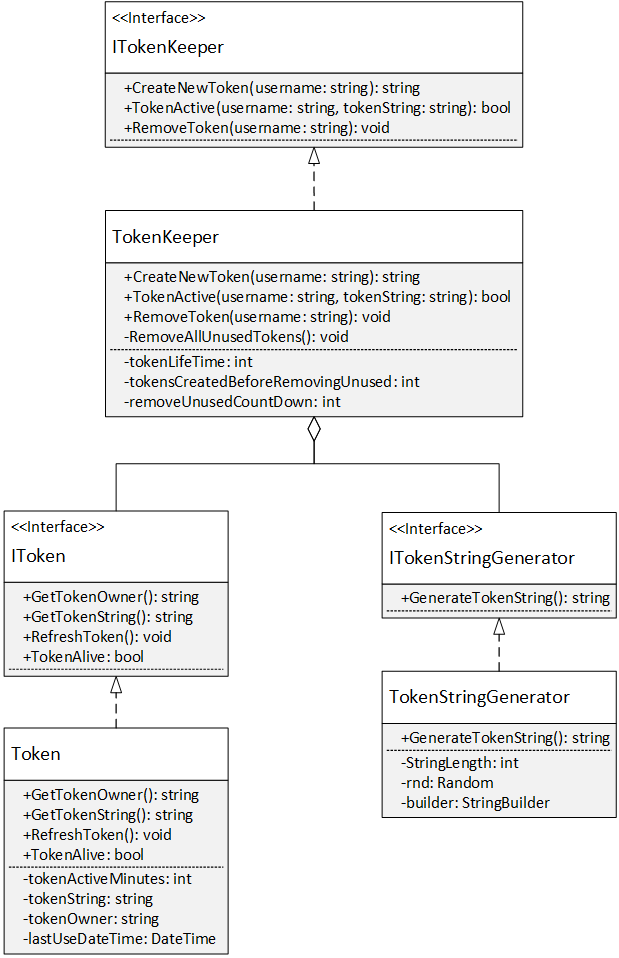
\includegraphics[width=0.7\linewidth]{figs/connection/ConnectionServerToken.png}
	\caption{Connection.Server.Token}
	\label{fig:ConnectionServerToken}
\end{figure}

For at simulere data fra pools i systemet, er der implementeret en række pool/sensor klasser. Disse ses på figur~\ref{fig:ConnectionPool}
\begin{figure}
	\centering
	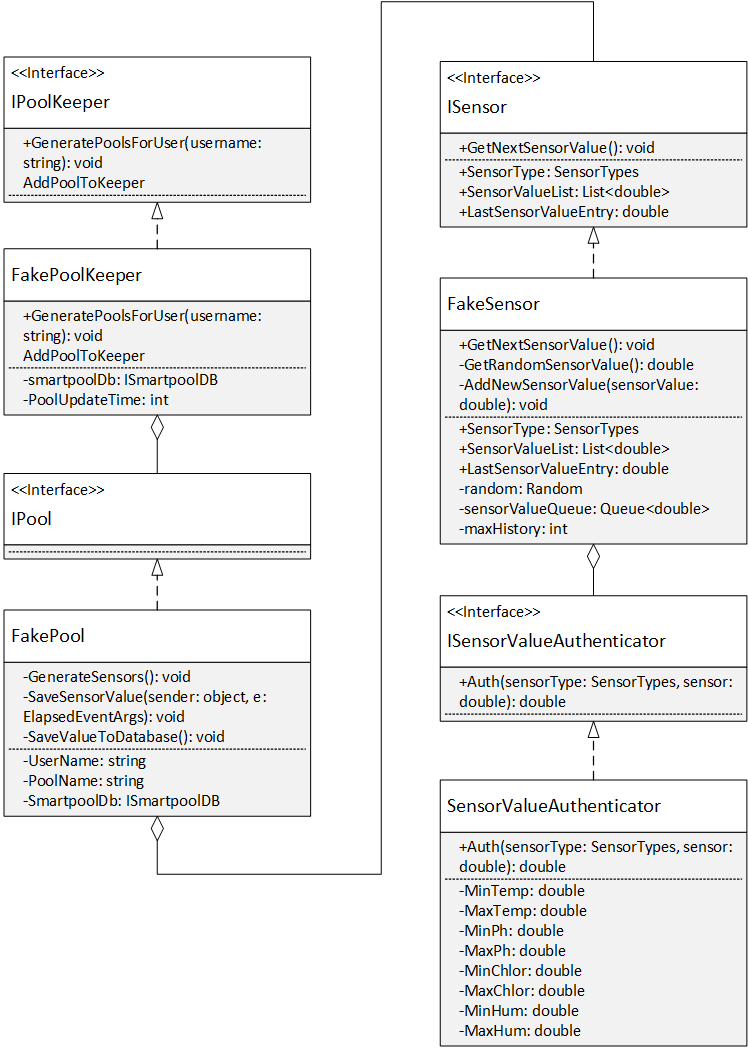
\includegraphics[width=0.8\linewidth]{figs/connection/ConnectionPool.png}
	\caption{Connection.Pool diagram}
	\label{fig:ConnectionPool}
\end{figure}

Klient og server kommunikerer med hinanden vha. en række besked objekter. Strukturen af disse er udarbejdet efter følgende diagrammer.

Nedarving fra message klassen er vist på figur~\ref{fig:MessageUML}
\begin{figure}
	\centering
	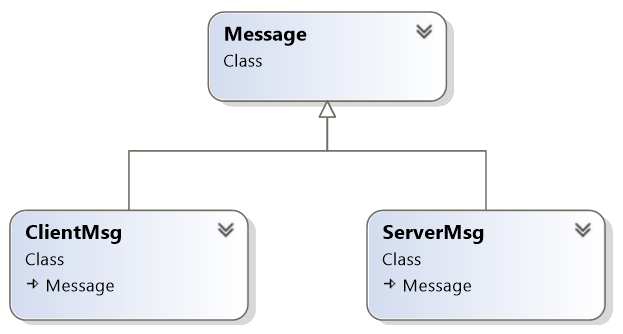
\includegraphics[width=0.6\linewidth]{figs/connection/MessageUML.png}
	\caption{Message nedarving}
	\label{fig:MessageUML}
\end{figure}

Nedarving fra ClientMsg klassen er vist på figur~\ref{fig:ClientMsgUML}
\begin{figure}
	\centering
	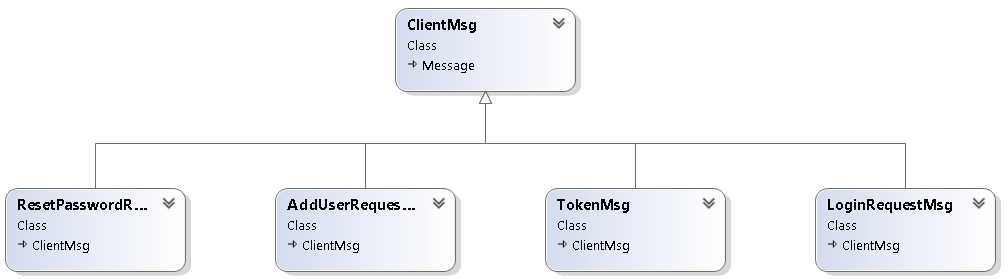
\includegraphics[width=0.9\linewidth]{figs/connection/ClientMsgUML.png}
	\caption{ClientMsg nedarving}
	\label{fig:ClientMsgUML}
\end{figure}

Nedarving fra TokenMsg er vist på figur~\ref{fig:TokenMsgUML}. AddPoolPictureRequestMsg er ikke blevet implementeret, men var en del af de user stories som blev udvalgt i starten af projektet, og er derfor taget med på figuren.
\begin{figure}
	\centering
	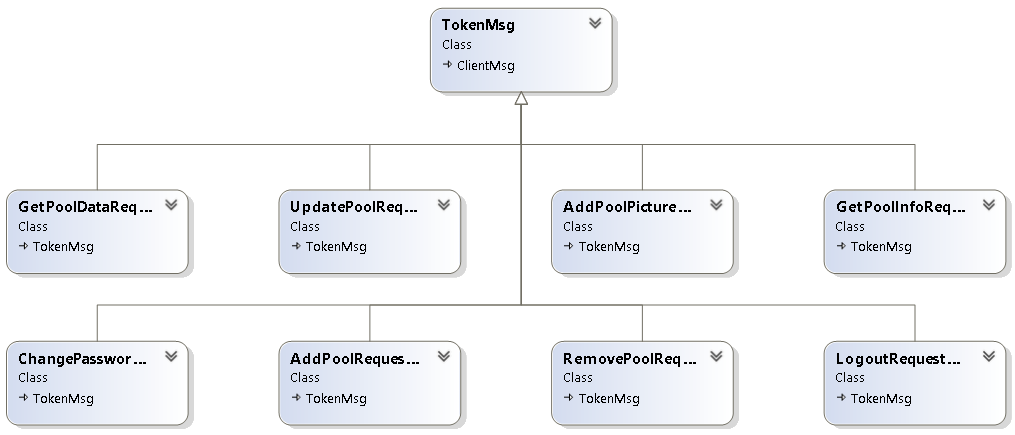
\includegraphics[width=0.9\linewidth]{figs/connection/TokenMsgUML.png}
	\caption{TokenMsg nedarving}
	\label{fig:TokenMsgUML}
\end{figure}

Nedarving fra ServerMsg er vist på figur~\ref{fig:ServerMsgUML}
\begin{figure}
	\centering
	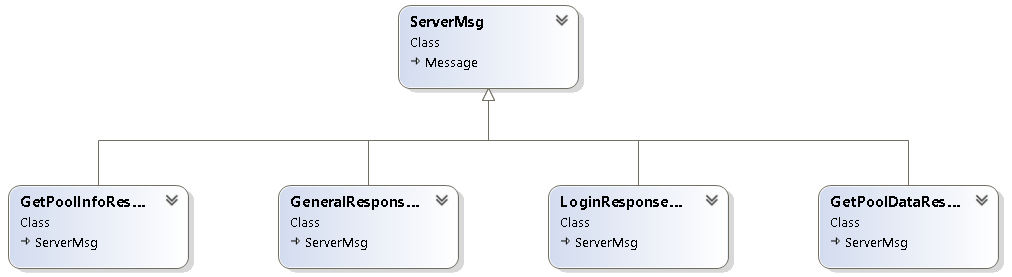
\includegraphics[width=0.9\linewidth]{figs/connection/ServerMsgUML.png}
	\caption{ServerMsg nedarving}
	\label{fig:ServerMsgUML}
\end{figure}

